\section{Discrete Fourier Transform}
\label{sec:DFT}
The computation of the FT will be done numerically. This can be done in a highly efficient algorithm called the Fast Fourier Transform (FFT). Using the Discrete Fourier Transform (DFT) it approximates the continuous FT of a function $g(x)$, where the FT of a two dimensional function is defined as
\begin{equation}
\hat{g}(f_X,f_Y)=\iint\limits_{-\infty}^{~~~\infty} g(x,y)e^{-j2\pi(f_Xx + f_Yy)}dxdy.
\end{equation}
A first approximation is restricting the integral to the finite interval $-L_x/2 \leq x \leq L_y/2$ and $-L_y/2 \leq y \leq L_y/2$, giving us, for $L=L_x=L_y$,
\begin{equation}
\hat{g}(f_X,f_Y)\approx\iint\limits_{-L/2}^{~~~L/2} g(x,y)e^{-j2\pi(f_Xx + f_Yy)}dxdy.
\end{equation}
Where the size $L_x$ and $L_y$ must be large enough to cover the essential non-zero parts of the function $g(x,y)$. Second the integral is approximated by replacing it by a finite sum, then we get
\begin{equation}
\hat{g}(f_X,f_Y)\approx  \Delta y \sum\limits_{m=N_y/2}^{N_y/2} e^{-j2\pi mf_Y\Delta y}\Delta x\sum\limits_{n=-N_x/2}^{N_x/2}g(n\Delta x,m\Delta y)e^{-j2\pi nf_X\Delta x },
\end{equation}
where the $x,y$-coordinates are sampled in the before described intervals with $N_x,N_y$ samples, when $N=N_x=N_y$, spaced at $\Delta x=\Delta y = L/N$ at positions $x_n=n\Delta x$ and $y_m=m\Delta y$ with $n=m=-N/2,...,N/2-1$. A connection to the DFT can be made by sampling the spatial frequencies with $N$ values in the interval $-\Delta x/2 \leq f_X \leq \Delta x/2$ and $-\Delta y/2 \leq f_Y \leq \Delta y/2$, the samples being spaced by $\Delta f_X=\Delta f_Y=1/L$ at frequencies $f_k=k\Delta f_X$ and $f_l=l\Delta f_Y$, with $k=l=-N/2,...,N/2-1$. This produces the exact DFT described by
\begin{equation}
\hat{g}(k\Delta f_X,l\Delta f_Y)\approx  \Delta y \sum\limits_{m=N_y/2}^{N_y/2} e^{-j2\pi lm/N_y}\Delta x\sum\limits_{n=-N_x/2}^{N_x/2}g(n\Delta x,m\Delta y)e^{-j2\pi kn/N_x}.
\end{equation}
In short the procedure is:
\begin{enumerate}
	\item sampling the function $g(x,y)$ in a grid at values $(x_n,y_m)$ and storing the values in a matrix of size $(N_x,N_y)$,
	\item doing a DFT on this matrix and multiplying it with the sample spacings $\Delta x$ and $\Delta y$,
	\item plotting the resulting matrix of size $(N_x,N_y)$ at points $(f_k,f_l)$ in the spatial frequency space.
\end{enumerate}
The numerical calculation of the diffraction pattern is now easily done by applying the FFT to $U_i(\xi,\eta)P(\xi,\eta)$ adding the multiplicative factor as seen in Equation \eqref{eq:fresnel} and setting $(f_k=\frac{x_k}{\lambda z},f_l=\frac{y_l}{\lambda z})$. The intensity distribution is then found by taking the modulus squared.

\subsection{Analytic and Numerical Solutions}
In figure \ref{fig:num_vs_an} the difference is seen between the numerical solved diffraction pattern and the analytically solved diffraction pattern. Clearly the two are almost identically except for the outer rings where the flaws of numerical computation are seen through the not disk like shape in the airy function. Because only the first few orders of the airy disk are important this is a good approximation to be used for calculating the centroids. 
\begin{figure}[H]
	\centering
		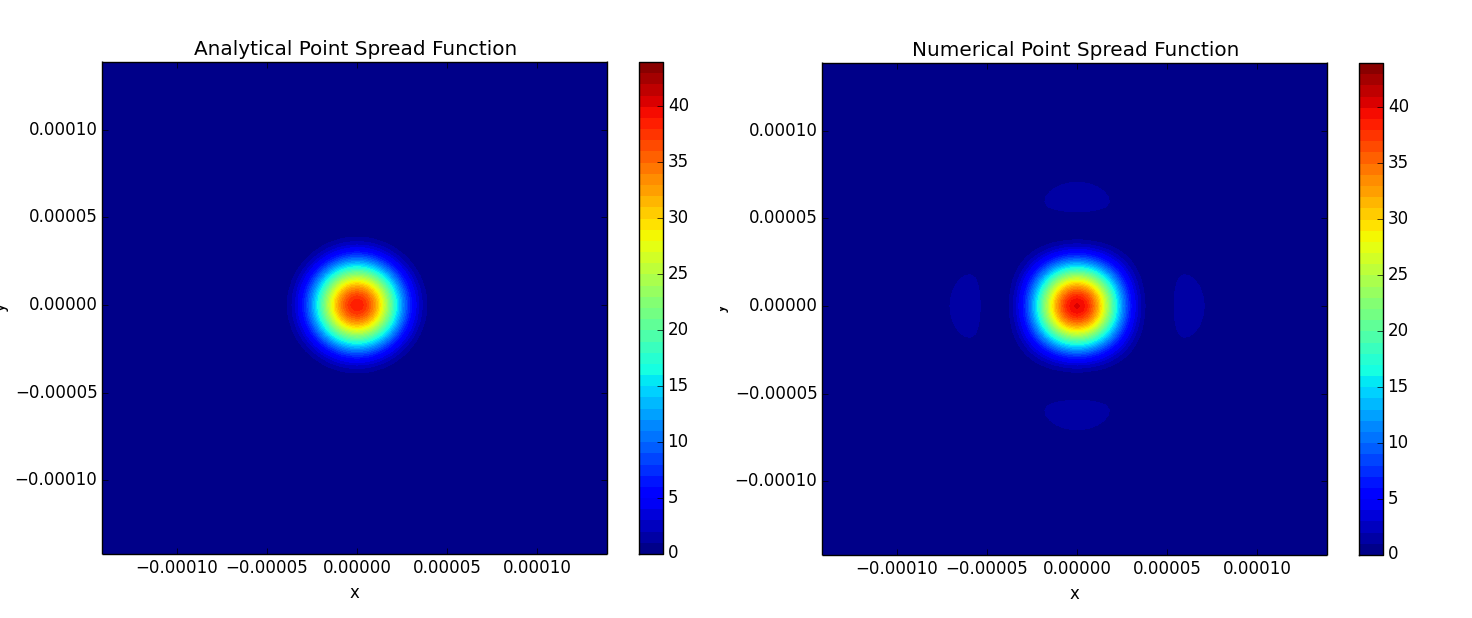
\includegraphics[width=1.0\textwidth]{figures/num_vs_an.png}
	\caption{Numerical solution VS analytical solution}
	\label{fig:num_vs_an}
\end{figure}

\subsection{Image Size and Sampling}
The selection of the size of the imaging plane and sampling plane have a large effect on the numerical solution when found through the DFT.  The more highly sampled, the more similar the numeric solution will be to the analytical solution.  


